% Created 2020-09-15 Tue 14:54
% Intended LaTeX compiler: pdflatex
\documentclass[9pt]{extarticle}
\usepackage[utf8]{inputenc}
\usepackage[T1]{fontenc}
\usepackage{tikz}
\usepackage{forest}
\usepackage{graphicx}
\usepackage{grffile}
\usepackage{longtable}
\usepackage{wrapfig}
\usepackage{rotating}
\usepackage[normalem]{ulem}
\usepackage{amsmath}
\usepackage{textcomp}
\usepackage{amssymb}
\usepackage{capt-of}
\usepackage[hidelinks]{hyperref}
% \usepackage{minted}
\usepackage[a4paper, total={6in, 9in}]{geometry}
% \setminted{breaklines, autogobble}
% \usemintedstyle{emacs}
\author{Nebhrajani A. V.}
\date{\today}
\title{\huge ZIO Select Answers}
\hypersetup{
 pdfauthor={Aditya V. Nebhrajani},
 pdftitle={IP OTBA Answers},
 pdfkeywords={},
 pdfsubject={},
 pdfcreator={Emacs 25.2.2 (Org mode 9.3.6)},
 pdflang={English}}
\begin{document}

\maketitle
% \tableofcontents

This document outlines my answers to some ZIO questions I found
interesting or instructive. The solutions are written the way I solved
them. In some cases, the solution is much better than the equivalent
given in answer keys, in others, the answer key does the job
better.

\section{2010}
\subsection{Org-Trees}

On first observation, the problem seems incredibly difficult to do
because of the sheer number of combinations one can achieve in large
org trees. The key insight, however, is that trees can (and should) be
seen recursively bottom-up, a technique in dynamic programming.

Consider the simple tree (direction of arrows is omitted where
hierarchies are obvious):
\begin{center}
  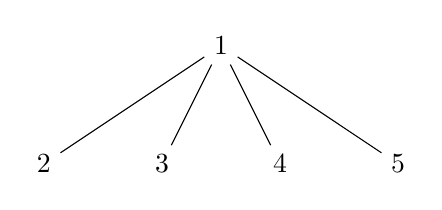
\begin{tikzpicture}
    \node {1} child {node {2}} child {node {3}} child {node {4}} child
    {node {5}};
  \end{tikzpicture}
\end{center}

In how many ways can we delete a leaf level node? Obviously,
only one way: just delete it. However, note that we always have the
option of \emph{not} deleting the node as well, giving us a total of 2
ways of dealing with leaves. Now, apply combinatorics. The total number of ways of deleting $1$ (or
below) will be the product of the ways of deleting its children, plus
one for its own deletion.

Therefore, writing number of ways of deletion into the tree:
\begin{center}
  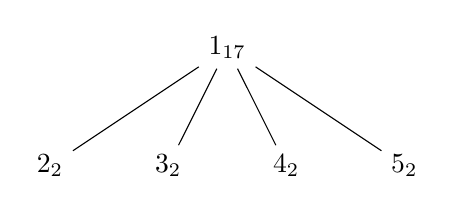
\begin{tikzpicture}
    \node {$1_{17}$} child {node {$2_2$}} child {node {$3_2$}} child {node {$4_2$}} child
    {node {$5_2$}};
  \end{tikzpicture}
\end{center}

And the problem is solved. Solving the first subproblem as an example,
\begin{center}
  \begin{forest}
    [1 [2 [5]] [3 [6 [10] [11]] [7 [12] [13] [14]]] [4 [8] [9]]]
  \end{forest}
\end{center}

Solving bottom-up:

\begin{center}
  \begin{forest}
    [691 [3 [2]] [46 [5 [2] [2]] [9 [2] [2] [2]]] [5 [2] [2]]]
  \end{forest}
\end{center}



\end{document}